%%%%%%%%%%%%%%%%%%%%% chapter.tex %%%%%%%%%%%%%%%%%%%%%%%%%%%%%%%%%
%
% sample chapter
%
% Use this file as a template for your own input.
%
%%%%%%%%%%%%%%%%%%%%%%%% Springer-Verlag %%%%%%%%%%%%%%%%%%%%%%%%%%
%\motto{Use the template \emph{chapter.tex} to style the various elements of your chapter content.}
\chapter{Introduction} \label{sec:intro}

\abstract{xxx}

\section{Typical On-Chip Faults} \label{sec:sec1.1}
To be added.

\subsection{Process Variation}
To be added.

\subsection{Manufacturing Defects}
To be added.

\subsection{Chip Aging}
The on-chip fault tolerance paradigm can help maintain the lifetime reliability of microprocessors suffering in-field degradation ascribed to both silicon devices and metal wires. The degraded silicon (including the devices and wires) is metaphorically called “Sick Silicon” \cite{yan2015corerank}. According to International Technology Roadmap For Semiconductors (ITRS) projection, silicon aging tops the impending (above 22 nm) reliability challenges. The industry and academic communities have performed significant work to understand the failure mechanisms of semiconductor devices, such as electromigration (EM), bias temperature instability (BTI) including negative and positive BTI (also known as NBTI and PBTI, respectively), time dependent dielectric breakdown (TDDB), hot carrier injection, and temperature cycling, etc. Both NBTI and TDDB draw the most attention concerning several transistor aging mechanisms. Both of them can gradually degrade performance over time. The researchers have evidence that circuit path delay can increase by 10\% during the five-year lifetime \cite{wang2007impact}. Even worse, with technology scaling to the nano-scale, the transistors tend to become more vulnerable and more prone to aging impacts \cite{wang2007impact}. 

The integrity of the wires is also degraded. The shrinking size leads to increased current density. Increased current density causes aggravated EM effects, which also contribute to the in-filed performance and reliability degradation. The effects of EM produce increased resistance of the wires and thereby result in increased RC delay. The increasing delay will eventually outgrow the timing margin and, even worse, the wires will eventually breakdown, causing break faults, bridge faults, or stuck-at faults in the chips. 

Since the whole chip is exposed to these aging mechanisms, some parts of the chip suffer faster aging than the others. The main reason can be attributed the following two aspects.

First, the “weak” chips, which are more sensitive to aging, mainly results from process variations \cite{borkar2003parameter}. As the feature size relentlessly shrinks generation-by-generation, the impacts of process variations become increasingly evident. Because of the wafer-to-wafer, die-to-die, and within-die variations, the proportion of the circuits with serious mismatches to the golden reference in the design print should be marked as weak silicon and removed from the production batch as yield loss. For example, the typical threshold voltage $V_{th}$ of transistors may exhibit obvious deviations from the standard settings because of width/length fluctuations caused by an unstable lithographic process. Those transistors with the elevated $V_{th}$ have smaller tolerances to withstand the aging induced $V_{th}$ increasing and are therefore prone to be more sensitive to it than those with larger tolerances.

Second, the aging rate of silicon devices (including the metal wires) depends not only on the intrinsic constitution of the devices themselves, but also on the stressing duty cycles [12]. From a microscopic perspective, the data patterns, which determine the BTI aging degree, are intrinsically non-uniform across the all bits. Consequently, some transistors are always positively or negatively-biased and therefore degrade much faster than those that are evenly-biased. The heavily-biased BTI aging has a slight chance to enjoy the recovery effect, which exacerbates the aging degree. From a microarchitectural perspective, for another example, the usage of some cores in a multicore processor could be always higher than the others because an oracle round-robin scheduling algorithm is not an option in modern operating system (OS) design. The jobs assigned to different cores can show very distinct stressing degrees. The computationally intensive jobs are usually more power-hungry and therefore generate more heat which can speed up the aging, while those computationally non-intensive jobs are the opposite.

\subsection{Soft Errors}
To be added.

\subsection{Intermittent Faults}
Intermittent hardware faults occur frequently and irregularly for a period of time, commonly due to manufacturing residuals, oxide degradation, process variations, and in-progress wear-out. Although intermittent faults and soft errors may manifest similar effects, there are several differences between them. First, from the spatial aspect, an intermittent fault occurs repeatedly at the same location, while a soft error rarely occurs in the same place. Second, from the temporal aspect, an intermittent fault will occur at burst, while a soft error is usually a single event upset or a single event transient. Third, if an affected structure has been replaced, intermittent faults will be eliminated; soft errors, however, can not be reduced by repair. There are also some differences between intermittent faults and hard faults. A hard fault exists during the lifetime of a chip and continually generates errors if the failing device is exercised, while an intermittent fault may be periodically activated and deactivated due to process and environmental variations. Intermittent faults also may turn to hard faults finally \cite{smolens2007detecting}.

An intermittent fault has three key parameters: burst length (BL), active time (AT), and inactive time (IAT) \cite{gracia2008analysis}. Burst length is the lifetime of an intermittent fault; active time is the positive pulse width of one activation, while inactive time is the time between two consecutive activations. The relationship among the three parameters can be expressed as $BL=N \times {AT} + (N - 1) \times IAT$ where represents the number of activations in an intermittent fault. These three parameters determine the characteristics of an intermittent fault, and their values can be dissimilar for different intermittent fault configurations. Figure \ref{fig:intermittent-faults} shows the temporal feature of intermittent faults within a period of time. Intermittent faults have adverse impact on program execution only during their active time. The time interval between two consecutive bursts is called safe time which means no intermittent fault occurs during that time, and the safe time could be varied because the occurrence of an intermittent fault is uncertain.

\begin{figure}[t]
\centering
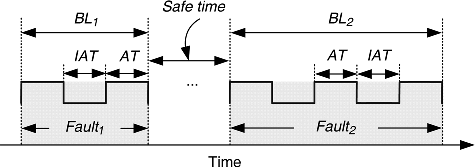
\includegraphics[scale=0.8]{IVF-fig1}
\caption{Key parameters of intermittent faults}
\label{fig:intermittent-faults} 
\end{figure}

In order to characterize the vulnerability of microprocessor structures to intermittent faults, it is important to establish appropriate logic fault models for them. The established logic fault models should represent physical intermittent abnormal phenomena that occur in real microprocessors. Based on the root causes and behaviors, intermittent faults can be classified into the following fault models \cite{gracia2008analysis} \cite{gil2003study}.

\begin{itemize}
    \item \textit{Intermittent stuck-at faults (including intermittent stuck-at-1 and stuck-at-0 faults):} Intermittent stuck-at faults are caused by residues in storage cells or solder joints during manufacturing. Unlike a soft error to upset a bit, an intermittent stuck-at fault transforms the correct value on the faulty signal line intermittently to be stuck at a constant value, either a logic value “1” or a logic value “0”. Structures most vulnerable to intermittent stuck-at faults are storage structures, such as memory and register file. In this work, we assume an intermittent stuck-at fault only causes one-bit of corruption.

    \item \textit{Intermittent open and short faults:} Intermittent open and short faults are usually caused by electro-migration, stress migration, or intermittent contacts. Intermittent open faults are breaks or imperfections in circuit interconnections such as wires, contacts, transistors and so forth. Intermittent short faults are shorts in wires or shorts in transistors. If an element being intermittently shorted to power or ground , it is equivalent to an intermittent stuck-at fault. If two signal wires are shorted together, an intermittent bridging fault occurs \cite{wang2006vlsi}. Figure \ref{fig:open-short-faults} illustrates several examples of intermittent open and short faults. The circuit consists of a two-input NOR gate and a NOT gate. is an intermittent open fault in transistor , while is an intermittent open fault in wire C. is an intermittent short fault to in wire D and is an intermittent bridging fault. Intermittent open and short faults may turn to hard faults if existing for a long time. Elements most vulnerable to these faults are signal buses and I/O connections.

    \item \textit{Intermittent timing faults:} Intermittent timing faults are mainly caused by inductive noises, aging, crosstalk, or process, voltage, temperature (PVT) variations. Intermittent timing faults will result in timing violations and affect data propagation when they occur. They usually lead to write wrong data to storage cells (i.e., flip-flops miss to latch the newly computed value due to path-delay) and finally become reliability problems. Intermittent timing faults can be broadly classified into intermittent path-delay faults and intermittent transition faults. In this work, we  mainly focus on intermittent path-delay faults. Besides, an intermittent timing fault may affect multiple bits of the data captured by storage structures or just a single bit in a structure. For example, a crosstalk induced delay fault may either affect multiple data lines or only one data line. We only consider the former situation that an intermittent timing fault affects multiple data lines.
\end{itemize}

\begin{figure}[t]
\centering
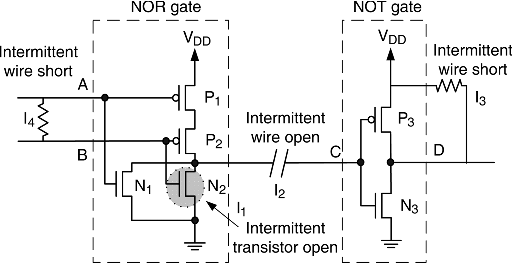
\includegraphics[scale=0.75]{IVF-fig2}
\caption{Examples of different intermittent open and short faults}
\label{fig:open-short-faults} 
\end{figure}

\begin{figure}[t]
\centering
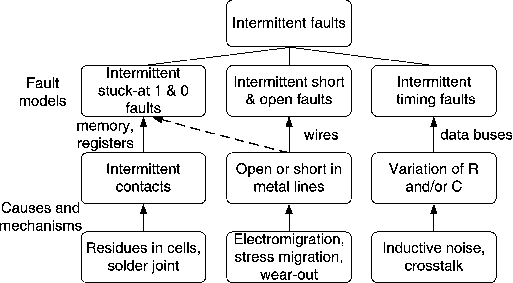
\includegraphics[scale=0.8]{IVF-fig3}
\caption{Physical causes, mechanisms, and fault models for intermittent faults}
\label{fig:fault-cause} 
\end{figure}


Figure \ref{fig:fault-cause} summarizes the main physical causes, mechanisms, and fault models for intermittent faults. Each kind of fault model has different causes, behaviors, and its own representative analysis method. Although the causes of these fault models may be different, they may have some physical causes in common. For example, the situation that an open or short in metal lines also can lead to intermittent stuck-at faults, such as the fault in Figure \ref{fig:open-short-faults}.

As we need to estimate the vulnerability of different microprocessor structures to intermittent faults, it is necessary to know the probability distribution of intermittent faults after establishing fault models. Srinivasan et al. \cite{srinivasan2005exploiting} show intermittent open and short faults obey log-normal distributions during the lifetime of microprocessors, which means the failure rate is low at the beginning of a microprocessor’s lifetime and it will grow as the microprocessor ages. Intermittent stuck-at faults and intermittent timing faults mainly obey uniform distribution and are highly dependent on the applications. To facilitate the analysis, we make the following assumption in this work: intermittent faults occur with high frequency and obey uniform distribution during program execution. The high intermittent fault rate is consistent with the public consideration of future industry technologies \cite{borkar2003parameter}. Although we only concentrate on the uniform distribution for intermittent faults, our evaluation methodology is also suitable to analyze other statistical distributions of intermittent faults.

\subsection{Emerging Technologies Induced Defects}
To be added.

\section{Conventional Wisdom for Fault-Tolerant Chip Design}
\subsection{Design for Test}
To be added.

\subsection{Design for Reliability}
To be added.

\section{On-Chip Fault-Tolerant Computing Paradigm}
Reliability is one of the mainstay merits of virtually any computing system. Beyond conventional fault tolerance computing \cite{degradation_05}, built-in on-chip fault tolerance faces several unique challenges: (1) Resource limited. On-chip fault tolerance is engaged during the duty time so that any dedicated automatic testing equipment (ATE) are unavailable. Therefore, the only viable strategy is to build all required test supports on the chip, which makes the on-chip fault tolerance mechanism operate in a self-supporting manner. (2) Overhead-sensitive. Even though silicon has become increasingly cheap thanks to the Moore's law, it is still unwise to extravagantly use the silicon for non-performance goals. For ordinary users, it is probably highly risky for the chip makers tout for customers with the probability of a system crash rather than the more appreciable performance.

Over the past decade, we have exploited the on-chip fault tolerance to build a holistic solution ranging from on-chip fault detection to error recovery mechanisms \cite{ReviveNet, fu2011abacus,  yan2015corerank, yan2010svfd, zhang2009topology, han2013revivepath, liu2021hyca}. We applied them to generic circuits, processing cores, Network-On-Chip
(NoC), deep learning processors. The on-chip fault tolerance framework usually consists of three key components: self-test, self-diagnosis, self-repair, or '3S framework' for short. Some prototypes have been built to demonstrate how on-chip fault tolerance responds to the in-filed silicon degradation. More interestingly, we find that the 3S framework is not only a powerful backbone guiding various on-chip fault tolerance designs and implementations, but also has more far-reaching implications such as maintaining graceful performance degradation, mitigating the impact of verification blind spots, and improving the chip yield. We believe that these design principles will be critical for the chip makers to maintain a competitive edge in the future.

As a fault tolerance mechanism, on-chip fault tolerance has the ingredients of generic fault tolerance mechanisms: fault detection, fault diagnosis, and fault recovery. Fault detection is used to judge whether the system suffers from erroneous executions, then fault diagnosis digs deeper to determine where and how such errors happen, which is followed by a recovery routine to correct the error to the expected outcomes. For the on-chip fault tolerance, the generic framework evolves with several new attributes which provide the essences of the self-supportive 3S approach.

\subsection{Self-Test}
The fault detection, which is virtually realized with dual-module redundancy either in spatial or temporal dimensions, is not viable due to its notoriously high overhead in terms of hardware or performance. For example, there are many fault detection schemes based on thread-level redundancy (TLR), core-level redundancy (CLR), and execution-level redundancy (ELR). Both TLR and CLR detect faults at the expense of computing throughput, a typical spatial dimension overhead. Furthermore, ELR virtually needs re-execution of the code and thereby dictates a large temporal overhead, even though such strict redundancy schemes promise perfect detection coverage.

To enable on-chip fault tolerance, we must resort to more thrift detection approaches. To achieve this, what we can compromise is the perfect detection coverage, given that the principal objective of on-chip fault tolerance is to isolate the Sick Silicon, rather than protect every instruction from fault contamination at all times. We design a highly cost-efficient self-test with respect to a probabilistic principle, rather than a deterministic principle. The detection routine should not take a significant number of processor cycles, and should be as transparent as possible to the kernel and user threads. Symptom-based fault detection which is built upon low-level circuit timing monitoring can fulfill this purpose \cite{yan2010svfd, wang2006restore}. 

\begin{figure}[t]
\centering
% Use the relevant command for your figure-insertion program
% to insert the figure file.
% For example, with the option graphics use
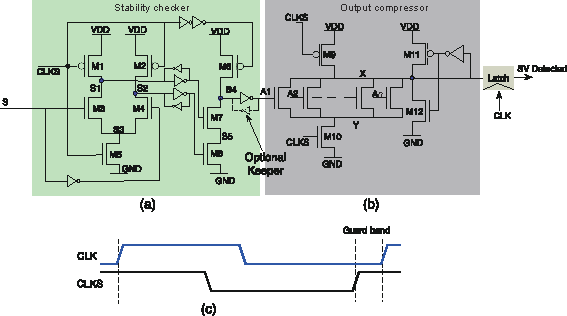
\includegraphics[scale=1.2]{fig1-2}
\caption{Timing sensor design. (a) stability checker; (b) output compressor; (c) clock timing.}
\label{fig:timing-sensor} 
\end{figure}


In symptom-based fault prediction, a symptom is defined as a signal stability violation. Basically, the stability violation of a signal is defined as at least one transition happens in the time interval during which the signal should be kept stable. A setup time violation, ascribed to progressive silicon aging for example, is a type of typical stability violation. As Figure \ref{fig:timing-sensor}(c) shows, in a clock cycle, we should reserve a timing span, that is a safeguard band, to meet the minimal setup time requirement. For the degradation-free case, there should be no single transition during the safeguard band; By contrast, if the transistors involved on the relevant timing paths suffer sufficient aging, the transition-free condition can no longer hold. By detecting the transitions in the safeguard band, the impending faults can be detected. Of course, whether an aged circuit can result in a stability violation is determined not only by the “sickness” of the silicon, but also by the data patterns which can sensitize the corresponding timing paths. However, the timing paths of Sick Silicon will show a much higher probability than healthy silicon to trigger the stability violations. By detecting the distribution of the stability violation, we can discriminate the sick parts from the healthy parts. 

The key instruments to detect the stability violation is timing sensors, which are commonly based on dynamic circuits satisfying sub-nanosecond to even tens of picoseconds detection resolution. Figure \ref{fig:timing-sensor} shows a sensor design. The basic stability checker (Figure \ref{fig:timing-sensor}(a)) can be derived from a sensing circuit for on-line delay fault detection, in which the integrity of the signal (S) is verified by a pair of exclusive nodes (S1 and S2), a stability violation will discharge the charged node and thereby cause both nodes to be at the “0” state, which signifies a timing violation. The outputs are compacted with a dynamic NOR for reducing the number of output latches (Figure \ref{fig:timing-sensor}(b)), where the M11 and M12 serve as a level restorer for node X. Multiple timing sensors are embedded in the host chip during fabrication. These sensors collectively form a monitoring system with fine-grained spatial detection resolution. The problematic component, such as an arithmetic logic unit (ALU), or a L1 cache bank, can be pinpointed. These faulty components can be masked from the other healthy parts, simply like a patient undergoes a surgery. These circuit-level adaptations can be automatically executed transparently on the host operation systems.

\subsection{Self-Diagnosis}
In on-chip fault tolerance, the diagnosis has two objectives: (1) pinpointing which components have been suffered permanent faults, and (2) estimating the level of performance degradation will be taxed due to the faults. Before delving into the details, we would like to first clarify the key differences between the built-in on-chip fault diagnosis and conventional chip diagnosis routines. The built-in on-chip fault diagnosis routine, called self-diagnosis, is very different from conventional diagnosis used in the yield learning phase, in terms of objective, techniques used, target granularity, and fault models.

\begin{itemize}
\item First, self-diagnosis is used to identify and locate the malfunctioning components, while the diagnosis in the production phase is mainly to help locate the defective physical or electrical contexts \cite{aitken2012yield}. The designers refine the physical designs to avoid these cases to ramp up the yield learning rate.

\item Second, the self-diagnosis intrinsically relies on built-in logic to locate the defective component, while the conventional diagnosis heavily relies on the silicon scan test and is conducted off-line by using sophisticated logical diagnosis tools.

\item Third, the granularity of self-diagnosis uses relatively coarse-grained components, such as core-level granularity, which have independent functionality and are usually loosely coupled with other parts, while the conventional diagnosis works at much finer-grained granularity at the logic gates or standard cells. In other words, self-diagnosis is based on functional testing and conventional diagnosis is based on structural testing.

\item Accordingly, the fault models of self-diagnosis describe the malfunction of components and therefore are more ad hoc, such as parity mismatch in the ALU components, while that of conventional diagnosis targets more silicon-level imperfections, such as bridge, open, abnormal leakage.
\end{itemize}

For on-chip fault tolerance, determining which parts of a chip get sick usually is trivial with the fine-grained self detection facility. If the corresponding timing sensors keep alerting stability violations, the faulty components can be switched off to avoid erroneous computations. In this case, the diagnosis and associated repairs are trivial. From Figure \ref{fig:self-diagnosis-example}, for example, there are four homogeneous ALUs in the processor core, the diagnosis agent logs the number of alarms reported by the self-test procedure. Each logging period can be as long as days or weeks to improve the diagnosis confidence level. By analyzing the alarm distribution, the self-diagnosis agent can discriminate the faulty ALU. In this example, the alarm density ascribed to ALU2 is significantly higher than the others, so the diagnosis agent marks that ALU2 should no longer be available anymore. The computation is thereby offloaded to the remaining three health ALUs. Consequently, this core will continue to work at the degraded performance level. The similar diagnosis logic can be also applied in the core-level, especially for many-core processors.

\begin{figure}[t]
\centering
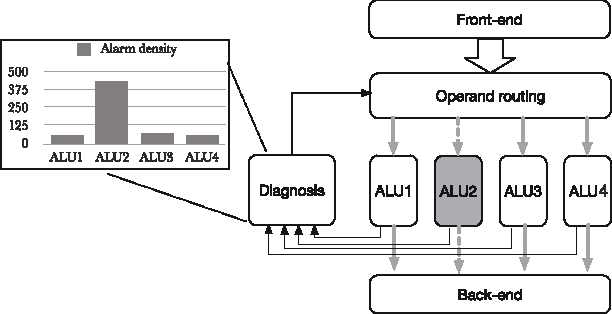
\includegraphics[scale=0.8]{fig1-3}
\caption{An self-diagnosis logic example for a 4-ALU processor.}
\label{fig:self-diagnosis-example} 
\end{figure}

It is more challenging to determine the performance impact given the faults detected, because the performance degradation depends on both the applications and the extent of the defects. For example, Figure \ref{fig:performance-degradation} shows the performance responses of the cores under various types of degradation. The cores are salvaged from instruction window defects, or L1 instruction/data cache defects, or L2 cache defects, respectively \cite{salvaging}. For simplicity, we do not show the more complicated compound defects. The degradation degree of “0” indicates defect-free, and 1/2 indicates half of the resource is unavailable, and so on. The results show that the performance response not only depends on the degree of degradation, but also exhibits to be highly application-specific. For example, the gobmk (a SPEC CPU2006 benchmark) in Fig \ref{fig:performance-degradation}(a) shows to be very resilient to the instruction window degradation; however, by contrast, the leslie3d and GemsFDTD are very sensitive to it. Such complexity is never unique for the instruction window only, but also to other resources, as exemplified in the other three sub-figures. Hence, even though the defect and associated defect level are accessible to the OS, we still have no ways to determine the level of performance impact such a degradation causes the running applications.

\begin{figure}[t]
\centering
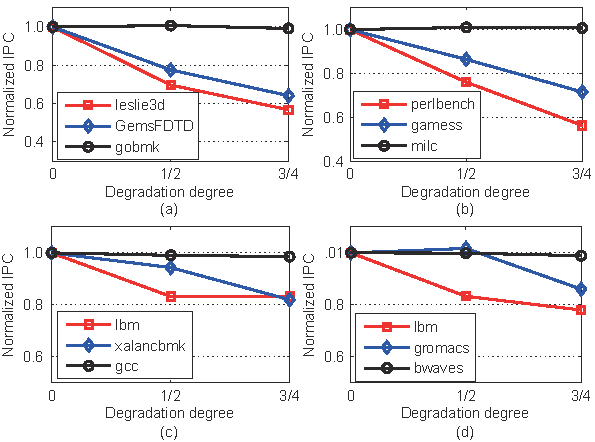
\includegraphics[scale=0.85]{fig1-4}
\caption{Performance degradation vs. defect degrees of (a) instruction window, (b) L1 instruction cache, (c) L1 data cache, (d) L2 cache, where the following SPEC CPU2006 benchmarks are used: leslie3d, GemsFDTD, gobmk, perlbench, gamess, milc, lbm, xalancbmk, gcc, gromacs, and bwaves.}
\label{fig:performance-degradation} 
\end{figure}


Yan et al. \cite{yan2015corerank} proposed the CoreRank approach to address this challenge. The CoreRank quantifies the core-level performance degradation towards more meta-program representations, called snippets, which are dynamic micro-operation streams and are oblivious to all the software level interference. The snippet can be readily characterized by built-in performance counters, without any instrumentation into the running workloads. The performance of core $C_i$ on the snippet $S_m$ is denoted as $P(C_{i}|S_{m})$, which can be obtained by reading the corresponding performance counters \cite{eyerman2007top}. If $P(C_{j}|S_{m})$ differs from $P(C_{i}|S_{m})$, the relative degradation can be easily extrapolated as the ratio of $P(C_{j}|S_{m})$ to $P(C_{i}|S_{m})$. Given any running program is composed of a sequence of various meta-programs (snippets), the program-level performance degradation can be estimated by aggregating the degradation on each individual snippet. Please refer to \cite{yan2015corerank} for more details.

For on-chip fault tolerance, the diagnosis is triggered only when the test procedure prompts the alarms. To minimize the overhead, one diagnosis agent can be shared by multiple timing sensors in a round-robin manner \cite{ReviveNet} controlled by a finite state machine. To minimize the penalty of power and performance in the fault-free scenarios, the diagnosis procedure is not always on, but is periodically invoked by abnormal states such as a machine crash.

\subsection{Self-Repair}
Generally there are two types of core-salvaging approaches: (1) Fault isolation. Decoupling the faulty components \cite{aitken2012yield} can avoid execution contamination and maintain a graceful degradation of performance. (2) Adaptive voltage-frequency setting and timing recycling \cite{tschanz201045nm}. For example, if the critical path delay increases due to aging, the functionality is maintained provided the working frequency is slowed down to accommodate the extra delay. The self-repair can be implemented at three abstract levels: circuit level, microarchitectural level, and architectural level. But we should note that such a classifying scheme is never strict, but only provides a roughly categorical image for easier understanding.

\subsubsection{Rejuvenation at the circuit level}
Figure \ref{fig:circuit-repair} illustrates a circuit-level pipeline with a rejuvenation facility. Each stage is monitored by a set of periodically-invoked aging sensors used to detect the signal transitions in the safeguard band. The aging sensors are deployed to monitor the critical paths. In the fault-free scenarios, no transitions could happen in the safeguard band, but after suffering from aging, some transitions could be delayed into the safeguard band, represented as a stability violation \cite{yan2010svfd}, a type of faulty symptom. With the awareness of aging, we can accommodate the impending aging failures by adapting localized timings. The adaptation to each stage is implemented with a set of time-borrowing agents which are fed by not only the local stages aging sensors but also the next stages agents, thereby enabling bidirectional adaptation, namely backward timing adaptation (BTA) and forward timing adaptation (FTA). The BTA uses the $(K + 1)$st stages timing slack to accommodate the aging emergencies in the $K$th stage, while the FTA uses the $(K1)$st stages slack to accommodate the emergencies in the $K$th stage. When an aging sensor detects an alarm, the BTA, FTA, or BTA and FTA can be simultaneously enabled to tolerate this aging delay.

\begin{figure}[t]
\centering
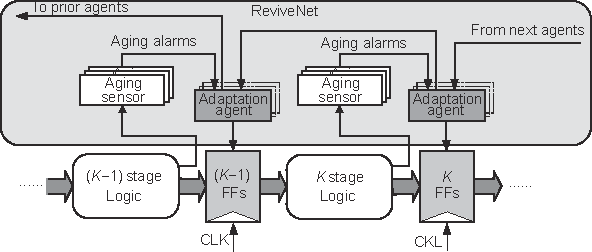
\includegraphics[scale=0.8]{fig1-5}
\caption{Circuit-level rejuvenation with timing adaptation.}
\label{fig:circuit-repair} 
\end{figure}


\subsubsection{Rejuvenation at the microarchitectural level}
The microarchitectural rejuvenation largely relies on decoupling the faulty components from the remaining healthy parts, or reconfiguring the microarchitectures \cite{salvaging}. The components which can be readily modified to be reconfigurable include the ALU arrays, cache banks, and register files. They share the common feature of regularity with intrinsic spares. The repaired procedure is also similar: marking the faulty component as unavailable so it will never be allocated to dynamic instructions. With some more sophisticated circuit techniques, these components can even be totally decoupled from the power grid, thereby preventing them from leakage.

For example, as shown in Figure \ref{fig:microarch-repair}, Core A and Core B suffered a pipeline defect and an L1 I-cache defect, respectively. The defect-affected partitions, marked as dark parts, are decoupled from the rest to make each core functionally correct, but in a degraded manner.

\begin{figure}[t]
\centering
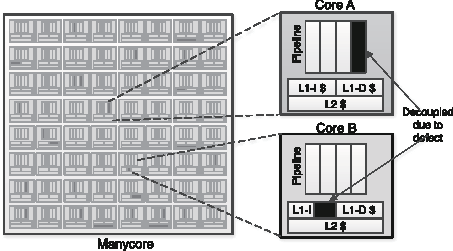
\includegraphics[scale=0.95]{fig1-6}
\caption{Microarchitectural rejuvenation.}
\label{fig:microarch-repair} 
\end{figure}

In fact, such microarchitectural approaches are more common in on-chip memory subsystems. A cache or scratchpad memory, always occupies a significant proportion of silicon real-estate. Using the last level cache for example as the failure mechanism in the SRAM cells, it suffers from different fault models, such as permanent read/write failures due to the SNR issue, retention fault or single-event upset (SEU). Regarding the granularity of the cache failures, it includes conventional bit failures and array or bank failures that occur in large-scale cache structures like distributed NUCA architectures. Fine-grained cache failures can be cured with conventional error correction or bit/row/column replacement. However, in modern large scale chip multi-processors, bank-level failures due to interconnection issue or isolation requirements are less discussed. For example, when a NoC-node is isolated from a resilient chip multiprocessor, it also creates inaccessible NUCA cache banks because of the connectivity issue, which should be tolerated to enable a degradable cache system. We propose a bank remapping method to cure the coarse-grained NUCA cache failure within the framework of self-test, self-diagnosis, self-fault-isolation. It utilizes the routing logic in NoC to transparently remapping the physical space associated to failed banks to healthy cache banks, so that the system will not see the cache failure and maintain a wholesome physical memory space on-chip. 

Furthermore, to reduce the negative impacts imposed by the bank failures, our work uses a utility-driven remapping policy to match the failed cache banks to an under-utilized cache bank, so that the system receives the least performance penalties caused by the bank failures. The remapping method relies on a dynamic stack-distance analyzer to measure the space utility of different address spaces and keeps on remapping the failed banks to their favored compatible healthy banks. In this way, the bank sharing induced block conflict will be reduced and the conflict-induced eviction cache miss rate will be minimized. The whole framework guarantees that the bank failure will be tolerated with a very small performance cost. When future systems are built with unstable devices or an unstable environment, such an inexpensive fault tolerant mechanism is very useful.

\subsubsection{Rejuvenation at Architectural Level}
The architectural rejuvenation is usually conducted at the core-level. There are two major rejuvenation styles: topology-invariant and topology-reconfigurable approaches, where the topology refers to the NoC topology connection of tens even hundreds of cores. 

Using core level DVFS to tolerate a cores degradation is a typical topology-invariant approach. The cores initially have the same maximum frequency, Fmax, but with the in-field aging degradation, the Fmax of the cores can differ from each other. If a core ages with a prolonged critical path delay, we can scale down the cores frequency to maintain safe timing, at the expense of more sophisticated per-core DVFS. Meanwhile, the topology, that is the cores location related to other cores, remains intact. 

The topology-invariance can simplify the NoC implementation and traffic management. However, if a core suffers an irreparable failure, we must either map it out of the healthy region, or find a substitute. In either case, the topology must be changed and topology-reconfigurable approaches must be employed \cite{fu2011abacus} \cite{zhang2009topology}. One typical solution is called N +M paradigm, i.e., there are N normal cores, which are visible to the OS, and M spare cores, which only serve as substitutes for failed cores and are invisible to OS. The similar solution is adopted in the “Cell” processor (N=7, M=1), where an N-core processor is provided with M redundant cores and we always provide customers with N operational cores. The spare cores are viewed as overhead. However, as the number of on-chip cores increases, the overhead of leaving a few redundant cores on-chip unused is acceptable because a single core is inexpensive compared to the entire chip. 

In fact, the industry has started to employ core-level redundancy in their products. Even though the objective is mainly for yield or performance, a similar rationale should be also applied to enhance the lifetime reliability. In such a case, rejuvenation is about substituting the faulty cores with the spares. The topology determines the ideal performance whereas the routing algorithm and the flow control mechanism determine how much of this potential is realized. However, when the failure cores are replaced by spare cores, the topology of the target design can be different. For example, suppose we want to provide 9-core processors with a 3×3 2D-mesh topology, as shown in Figure \ref{fig:topology-reconfig}(a). Also, suppose three redundant cores (1 column) are provided, as shown in Figure \ref{fig:topology-reconfig}(b). If some cores (no more than three) are defective, we could still get 9-core processors. 
However, from Figure \ref{fig:topology-reconfig}(c), if the faulty cores are replaced by the spare cores, not only are the topologies different from what we expect, but also the topologies of different chips can be very distinct. Consequently, there is a mismatch between the logical topology, 2D-mesh in this example, and the physical topology, namely the topology with the disabled cores. Clearly, there could be many ways to map the logical topology to the physical topology. So, the challenge in the N + M paradigm is to determine which topology is optimal. The problem has been proven to be NP-complete and can only be solved with a heuristic algorithm \cite{zhang2009topology}.

\begin{figure}[t]
\centering
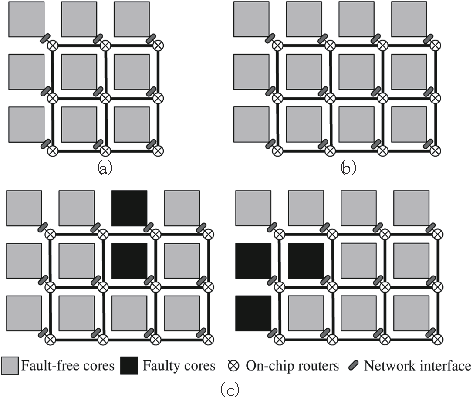
\includegraphics[scale=0.95]{fig1-7}
\caption{Topology reconfiguration-based architectural level rejuvenation for a manycore. (a) The topology demand;
(b) the topology with spare cores; (c) the topology with faulty cores.}
\label{fig:topology-reconfig} 
\end{figure}

\subsection{General Benefits}
The on-chip fault tolerance computing paradigm has great potential to critically complement the state-of-the-art IC designs. However, we should note that the specific techniques mentioned above should not be supposed to be comprehensive, but the concept of the 3S-based on-chip fault-tolerant design framework can be tailored for more purposes. We summarize three perspectives in the following section.

\subsubsection{Maintaining graceful degradation}
Faults could happen during the lifetime of a system. If the faults are transient, the system may be recovered by rebooting. However, if the faults are permanent, some resources of the system, such as cores in multi-core processor or interconnections of NoC will no longer be functionally correct. Without isolating the faults, the whole system may even turn off completely. However, by detecting, diagnosing, and isolating the faulty components, the system may still be able to work correctly using the remaining good components, though at a lower performance degree, i.e., Graceful Degradation. No redundant components are assumed, which means the components of the system have already satisfied the capability of reconfiguration for correct function. It is not surprising that these two design philosophies converge since they share the same objective. There are two key questions required to be answered for the on-chip fault tolerance computing paradigm based graceful degradation: (1) what is the granularity? (2) how to implement it? The on-chip fault tolerance computing paradigm sheds light on the answers.

The processor core and the NoC interconnection are two typical reconfigurable components used in graceful degradation. In multi-core processors, when one core is faulty, other cores can still function. In the NoC, when one interconnection node is faulty, other nodes may substitute its routing function. With on-chip fault tolerance, there are more redundant resources to keep the whole system working properly. More fine-grained components can also be considered. For example, a redundant arithmetic logic unit (ALU) can be added to a core, so when one ALU fails, the core can still work correctly.

Using more fine-grained components for fault tolerance and performance degradation can improve the lifetime of the system, but its disadvantage is the hardware cost, not only including the hardware for isolating the faulty components, but also including the hardware of detecting such fine-grained components. However, FPGA is an exception, since it is programmable. Hence detecting the faulty Look-Up Tables (LUTs), interconnection boxes, or other fine-grained components of FPGA can be realized by specific circuits, and isolating the faulty resources can be achieved using placement and routing constraints while designing FPGA circuits. Hence, it is possible for FPGA to perform fine-grained analysis without any hardware overhead, but with a performance penalty.

Furthermore, on-chip fault tolerance computing paradigm provides more possibilities and opportunities for effective graceful degradation. The implementation of graceful degradation requires accurate diagnosis of the faulty components. For example, in NoC, it is necessary to diagnose the switch, the router, the link, and so on \cite{kohler2010fault}. With the knowledge of locating the faulty components, the routing for graceful degradation is an optimization process with the constraint that the faulty interconnections should not be used. With more faulty components, more constraints exist in the optimization problem, so its solution, i.e., the performance, will become progressively worse, until it reaches a limit that no available routing can be found, and then the whole system will fail. 
Moreover, on-chip fault tolerance computing paradigm can make the graceful degradation more simplified and effective. If an interconnection node has two routers, one of which is redundant, then when the working router fails, the node can simply switch to the redundant one. In this case, the routing delay remains similar, so the performance is maintained.

\subsubsection{Helping fix some verification blind spots}
Modern designs have become more complicated, which poses serious challenges for verification. The verification techniques cannot scale to the complexity of the modern designs, so some bugs could escape from verification and remain in the silicon. If the bugs really exist, they are like permanent faults. If these faults are not detected during testing, the products with bugs will enter the market. If the bugs are encountered by customers, it will be a large financial loss to recall the chips. In this situation, On-chip fault tolerance computing paradigm is an alternative method to fix the problem. On-chip fault tolerance computing paradigm has at least two benefits for verification: (1) locate the verification blind spots; and (2) fix the escaped bugs.

From the perspective of behavior, the escaped bugs are like permanent faults. Both cause the system to work incorrectly. In on-chip fault tolerance computing paradigm, the preliminary step for isolating faults is to detect and diagnose the faults. The same function is suitable for finding the escaped bugs. Learning how and why the bugs escaped from the adopted verification techniques is important for improving the verification process and avoiding the similar bugs remaining in silicon. A more fine-grained fault detection can provide more precise information about the escaped bugs. For example, it is easy for the designers to learn the escaped bugs by informing them just the ALU is faulty than informing them the whole processor core is faulty.

Therefore, the detection circuit for escaped bugs should be designed properly. For example, the detection circuits can be inserted in some critical points in the control flow \cite{gizopoulos2011architectures}. Within the on-chip fault tolerance computing paradigm, the faults are isolated to allow the whole system to work correctly. Some bugs can also be isolated. However, since the bugs may be repeated, isolating the bugs may not be effective. For example, in the multi-core processor, if all the cores have the same design, they will contain the same bugs as well, so it is meaningless to isolate faulty cores. 

Under this scenario, there are three ways to correct the bugs. First, heterogeneous cores can be designed so that even if one type of core contains bugs, other types of cores may still function correctly by isolating the faulty cores. But this method may result in a large performance losses, since a portion of the cores are unavailable. Second, during the design, combined with fine-grained bug detection circuits, some configurable components can be inserted into the critical locations \cite{alizadeh2010debugging}. If bugs are detected, specific configuration bits can be downloaded to the configurable components to correct the circuit behavior. Furthermore, in the CPU+FPGA SoC, if some bugs exist in the computing components, it is also possible to use the FPGA as a fault-tolerant component to perform the correct function. Third, for some bugs, it is also possible to use software-hardware cooperation to bypass the bugs \cite{chang2011constraint}. For example, if there is a bug in the subtraction computation hardware component, the OS can compile a subtraction operation into an add operation. In this way, the same function is performed by detouring the bugs. Therefore, using the above methods, with properly inserted bug detection and recovery design, some escaped bugs from the verification phase can still be fixed after the chips are manufactured and sold to the customers, though with some performance degradation.

\subsubsection{Improving gross yield}
Bugs may escape from verification, and defects may happen during manufacturing. There are mainly two types of defects: the permanent defect and the transient defect. The permanent defects such as stuck-at faults will permanently affect the behavior of the chip. More specifically, they destroy the Boolean relation within the chip. In certain situations, the chip or the corresponding component will definitely fail. The transient defects, such as small delay defects, are types of timing faults. The chip only fails under a certain condition. Different from bugs which may be repeated, e.g., in multi-core processors, the cores with the same design have the same bugs, the defects do not have such characteristics. Hence the on-chip fault tolerance computing paradigm can also tolerate some defects. The chips with defects are considered as faulty chips, but if the defects can be tolerated, then the chips can still work correctly and be considered as good chips. Hence, the yield can be improved, but the promised performance may be degraded.

\section{Summary}
The proposed on-chip fault tolerance computing paradigm is an incorporative framework to build synergy among many advanced fault tolerance-oriented techniques. In this paper, we placed self-test, self-diagnosis, and self-repair (self-recovery) into a unified framework, namely the “3S” framework, and clarified the difference from their conventional counterparts whenever possible. We use the manycore undergoing various degrees of aging faults as the baseline to show the efficacy of on-chip fault tolerance, and discuss three far-reaching implications in terms of graceful degradation, verification, and yield. Although we have made some initial attempts to solidify this framework, the potential has never been fully exploited. We believe on-chip fault tolerance can help deliver more reliable SoC systems suffering in-field degradation in the future.

\bibliographystyle{plain}
\bibliography{refs}


